\documentclass{../iot-lecture}

\subtitle{IoT Platforms}

\addbibresource{main.bib}

\begin{document}

\begin{frame}
  \titlepage{}
\end{frame}
\begin{frame}
  \frametitle{Outline}
  \tableofcontents{}
\end{frame}

\section{IoT Platforms, What \& Why?}

\begin{frame}
  \frametitle{Challenges\footfullcite{Rub2020}}
  \begin{itemize}
    \item Lack of a common date format and sharing standard.
    \begin{itemize}
      \item Two different sensors can monitor the same parameter using different unit of measure.
    \end{itemize}
    \item Heterogeneity in networking and sensor technologies.
    \begin{itemize}
      \item Heterogeneous environment of IoT devices/plaforms that must be integrated into an interoperable one.
    \end{itemize}
  \end{itemize}
\end{frame}

\begin{frame}
  \frametitle{Challenges (Cont'd)}
  \begin{itemize}
    \item Lack of a standardized definition of environmental indicators.
    \begin{itemize}
      \item Standard doesn't consider clear metrics for water quality (i.e., temperature, pH, conductivity, and dissolved oxygen indicators)
    \end{itemize}
    \item Semantic interoperability between IoT solutions for the environment domain.
    \begin{itemize}
      \item Environmental studies can comprehend many phenomena through the observation/analysis of different features
        (i.e., earthquake can be predicted by vibrations or satellite image processing).
      \item A platform for environment studies must model and explore the semantic relation between heterogeneous data sets.
    \end{itemize}
  \end{itemize}
\end{frame}

\begin{frame}
  \frametitle{What is an IoT platform?}
  \begin{block}{Internet of Things Wiki\footfullcite{Top20IoTPlatforms}}
    In simple words the purpose of any \textbf{\color{YellowOrange} IoT device} is to connect with
    other IoT devices and applications (cloud-based mostly) to relay
    information using internet transfer protocols.

    The gap between the device sensors and data networks is filled
    by an \textit{\color{Green} IoT Platform}.
  \end{block}
\end{frame}

\begin{frame}
  \frametitle{What is their job?}
  \begin{itemize}
    \item Developers can develop their applications with ease
    \item End-users can see his/her dashboard and customize it
    \item The government can provide regulation on data
  \end{itemize}
\end{frame}

\begin{frame}
  \frametitle{Three-Layer IoT Architecture\footfullcite{Rub2020}}
  \begin{figure}
    \centering
    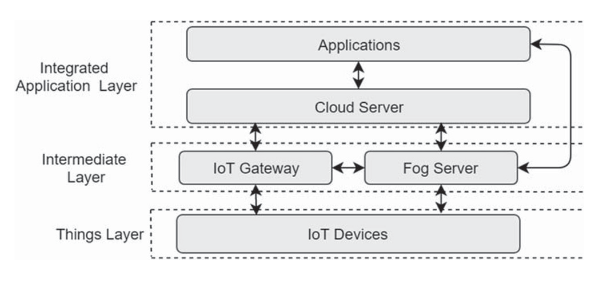
\includegraphics[width=\textwidth]{./img/three-layer-iot-architecture.png}
    \caption{structure of a three-layer IoT architecture}
  \end{figure}
\end{frame}

\begin{frame}
  \frametitle{Platforms' Components\footfullcite{Rub2020}}
  \begin{itemize}
    \item \textbf{\color{Cyan} Applications} processes the gathered environment data, apply data mining and other big data
      techniques, train complex machine learning models, or keep monitoring the data to support decisions.
    \item \textbf{\color{YellowOrange} Cloud Server} provides the platform features required for data storage and processing to support
      the data used by applications.
    \item \textbf{\color{LimeGreen} IoT Gateway/Fog Server} primarily function as a data relay between IoT Devices and Cloud Server.
    \item \textbf{\color{RubineRed} IoT Devices} measure the environmental parameters and forward the measures to the gateway or fog server.
  \end{itemize}
\end{frame}

\section{SenML}

\begin{frame}
  \frametitle{Sensor Measurement List (SenML)}
  \begin{itemize}
    \item Format specification for representing simple sensor measurements and device parameters.
    \item Representations are defined in
    \begin{itemize}
      \item Javascript Object Notation (JSON)
      \item Concise Binary Object Representation (CBOR)
      \item Extensible Markup Language (XML)
      \item Efficient XML Interchange (EXI)
    \end{itemize}
  \end{itemize}
\end{frame}

\begin{frame}[fragile]
  \frametitle{SenML in Action}
  \begin{minted}[bgcolor=Black]{json}
[
  {
    "n":"urn:dev:ow:10e2073a01080063",
    "u": "Cel",
    "v": 23.1
  }
]
  \end{minted}
\end{frame}

\begin{frame}
  \frametitle{SenML in Action (Cont'd)}
  \begin{itemize}
    \item Temperature gauge encoded in the JSON syntax
    \item The array has a single SenML record
    \item sensor's name is \textit{``urn:dev:ow:10e2073a01080063''}
    \item sensor's value is \textit{23.1 degrees Celsius}
  \end{itemize}
\end{frame}

%\begin{frame}[allowframebreaks]
%  \printbibliography%
%\end{frame}

\end{document}
